\section{Problem Context}
\subsection{UK Statistics}
In the UK alone, around 2,000,000 people live with sight loss --- around 360,000 of which are registered with their local authority as being blind or visually impaired, who have severe and irreversible sight loss~\cite{uk-blind}.  Of these 360,000 people, there are only 17,000 white cane-users, and less than 4,800~\cite{guidedog-count} guide-dog owners. Assuming no overlap between guide dog users and white cane users, this leaves almost 94\% without access to the two major forms of assistance available to the blind.

A possible factor that could explain the relatively small adoption of Guide Dogs is their cost --- as mentioned in section \ref{chap:introduction}, the life-time cost of a guide dog is around \pounds50,000. Although the dog is paid for in it's entirety by the Guide Dogs for the Blind association, they themselves are a charity and do not receive government funding. A system whereby the visually impaired could purchase a guide-dog would likely not be effective, as 66\% of the registered blind/partially sighted are not in paid employment~\cite{afbff} so would be unlikely to be able to afford the cost.

\subsection{Developing Countries}
The situation in less developed countries than the UK is far worse. According to the Himalayan Cataract Project~\cite{worldblindness}, ``blindness is most prevalent in developing countries where malnutrition, inadequate health and education services, poor water quality and a lack of sanitation leads to a high incidence of eye disease''. If these countries are so impoverished that they are unable to afford services that are considered basic human rights in the developed world, it is unlikely that they will be able to afford to spend \pounds50,000 per person on guide dogs. 

Although white canes are a cheaper, they are not without their downsides. They have limited range - typically a few feet in-front of the user. This makes finding doorways etc a more difficult task than when using a guide-dog.

\section{The Problem}
This project aims to address the lack of a cheap, intuitive way of enhancing the mobility of the visually impaired.

It is non-trivial to convey visual information in the form of audio, for a number of reasons.

\subsection{Compression}
\label{sec:compression}
Measuring the bit-rate of sensory systems is not an easy task --- however, research has been done into the informational capacity of both the human visual system, and human auditory system.

Evidence makes it clear that the human visual system has a higher bit-rate than the human auditory system. Estimates by H. Jacobson~\cite{jacobson1950informational} suggest the informational capacity for the human ear to be roughly $8\times10^3$ bits/sec. In a separate paper~\cite{jacobson1951informational} Jacobson also estimates the informational capacity of the human eye to be around $4.3\times10^6$ bits/sec --- roughly $\times500$ higher. 

Taking this into consideration, it is clear that a working solution to the problem that this project aims to solve will involve compression of the visual information. 

\subsection{Neuroplasticity}
Neuroplasticity is a term used to describe the ability of the brain to adapt to change. The brain is able to ``re-wire'' itself in response to changes to input, environment and emotions --- however, this process takes time, and deteriorates with age\cite{park2013aging}. Some existing solutions (see section \ref{sec:existing})

\ac{WHO} figures state that of the 39 million blind on planet, 82\% of those are aged 50 and above,

With this in mind, an inclusive, wide-reaching system should be as intuitive and natural as possible, and should not be too heavily reliant on neuroplasticity.

\section{Existing Solutions}
\label{sec:exisiting}
Several attempts to solve the problem of video to audio conversion have been made in the past.

\subsection{vOICe}
The technique described as "An Experimental System for Auditory Image Representations"~\cite{vOICe} sonifies an object/scene by producing a 1:1 mapping from image to audio. This is accomplished by generating a sound, such that a visualisation of the frequency spectrum of the sound produces the input image. This technique has been used by the artist Aphex Twin in the song $\Delta M_i^{-1} = - \alpha \sum_{n=1}^N D_i \left[ n \right] \left[ \sum_{j \in C \left[ i \right]}^{} F_{ji} \left[ n -1 \right] + Fext_i \left[ n^{-1} \right] \right]$~\cite{aphex-equation} (more commonly known as [equation]), where viewing the song in a spectrogram produces a picture of the artists face:

\begin{figure}[H]
    \centering
    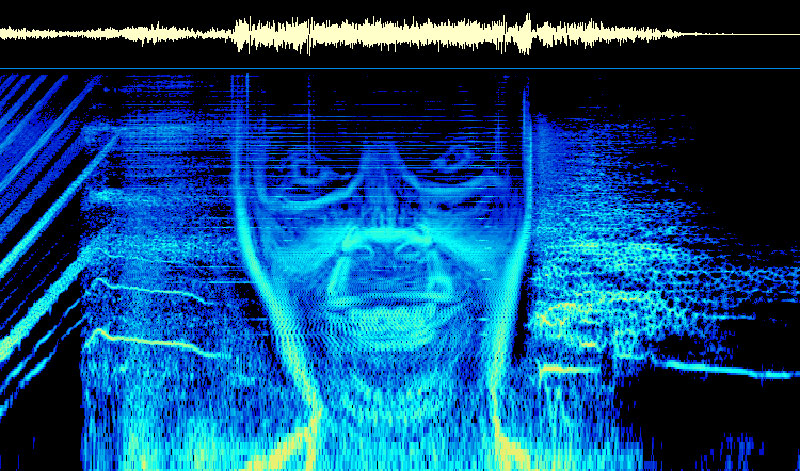
\includegraphics[width=\textwidth]{Background/equation-face.jpg}
    \caption{Spectrogram of $\Delta M_i^{-1} = - \alpha \sum_{n=1}^N D_i \left[ n \right] \left[ \sum_{j \in C \left[ i \right]}^{} F_{ji} \left[ n -1 \right] + Fext_i \left[ n^{-1} \right] \right]$~\cite{aphex-equation}}
\end{figure}

While this approach can theoretically convey all of the information held within the image, in practice, it is not feasible as a human visual aid. This method would require a human to perform a \ac{FFT} of the signal and re-construct the image in their head, and assumes that the auditory system has a sufficiently high bit-rate to receive all of the information, making the system unworkable --- little compression is performed. 

\subsection{Virtual Acoustic Space}
\label{sec:vas}
A paper by Gonzalez-Mora, J.L. et al~\cite{vas} describes a method involving \ac{VAS}. \ac{VAS} works by simulating the sound that a user would hear if a point source at a particular angle and distance from the user was emitting a tone. For each frame, several points are placed --- the field of view of the camera is divided into a $17\times9$ grid, with a point inserted in each division. 

The system is not totally dissimilar to echo-location, but uses a simulated response from the objects, rather than relying on an ultrasonic echo.

\begin{figure}[H]
    \centering
    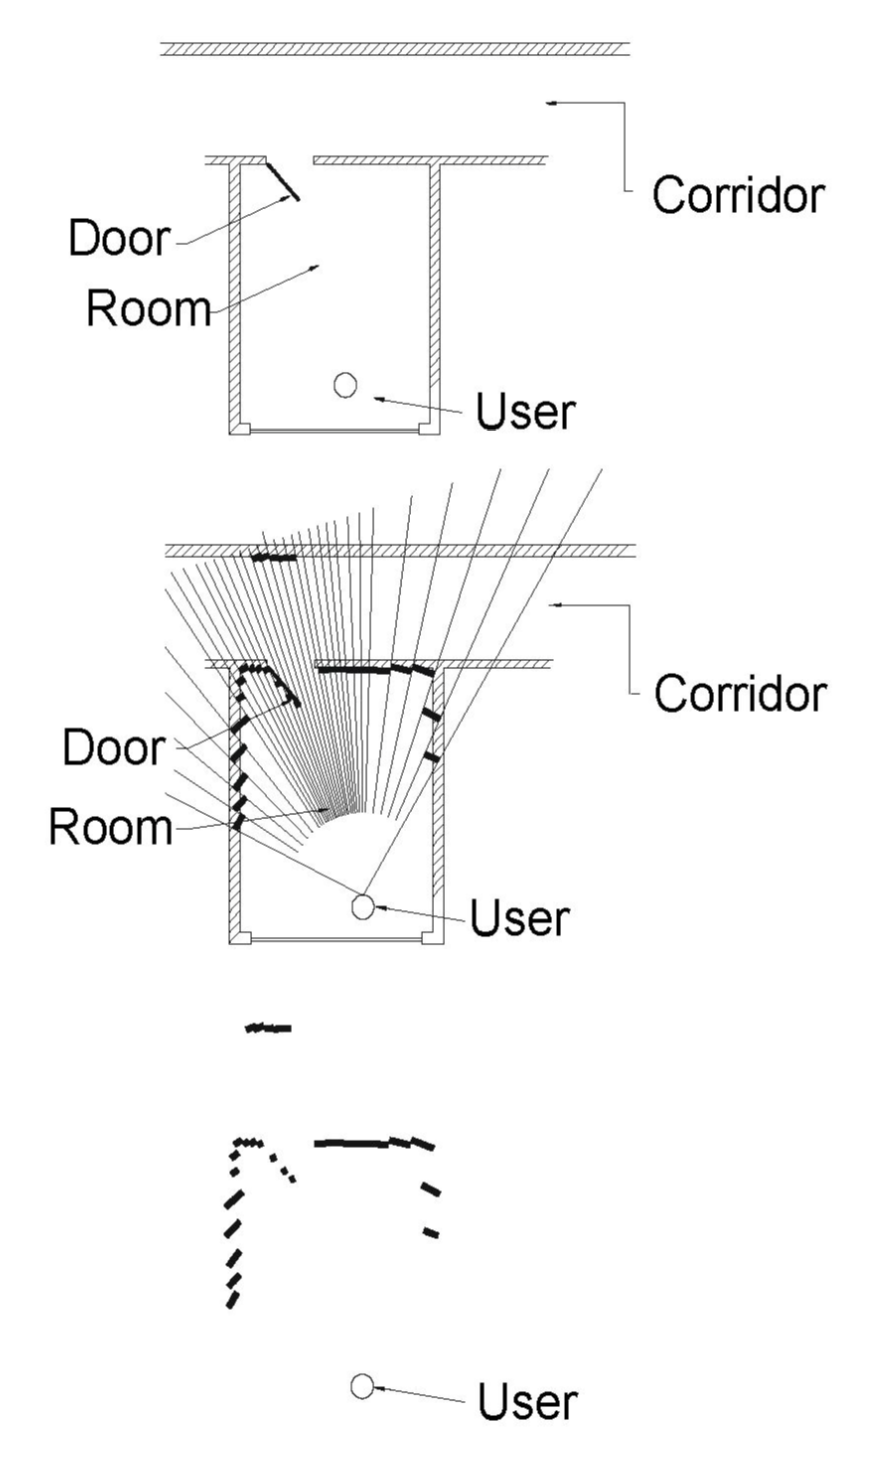
\includegraphics[width=0.5\textwidth]{Background/vas.png}
    \caption{Point placement with \ac{VAS}}
\end{figure}

The system described uses the \ac{HRTF} technique to apply filters to a tone. \ac{HRTF} works by modelling the effect the human body/head has on incoming audio. For instance, a tone emitted from a source to the left of a user has different properties when received on the left ear to the right ear; Higher frequencies will be attenuated more on the right ear, and there will be a slightly delay between the signal reaching each the right ear-drum compared to the left ear-drum. The \ac{HRTF} is applied to every point placed by the \ac{VAS} algorithm on both left and right channels. The modified tones (referred to as pips) are then played back in a random order. By inferring the position of each point based on it's acoustic properties, it has been shown that a trained user can navigate around a room.

\begin{figure}[H]
    \centering
    \includegraphics[width=0.25\textwidth]{Background/HRTF.png}
    \caption{Basis of HRTF technique~\cite{hrtf-diagram}}
\end{figure}

Although this system seems fairly effective, it is not without limitations.  

\subsection{TheVIBE}
``TheVIBE'' is a visuo-auditory sensory substitution system~\cite{thevibe}, which is similar in ways to the method discussed in section \ref{sec:vas}.

\begin{figure}[H]
    \centering
    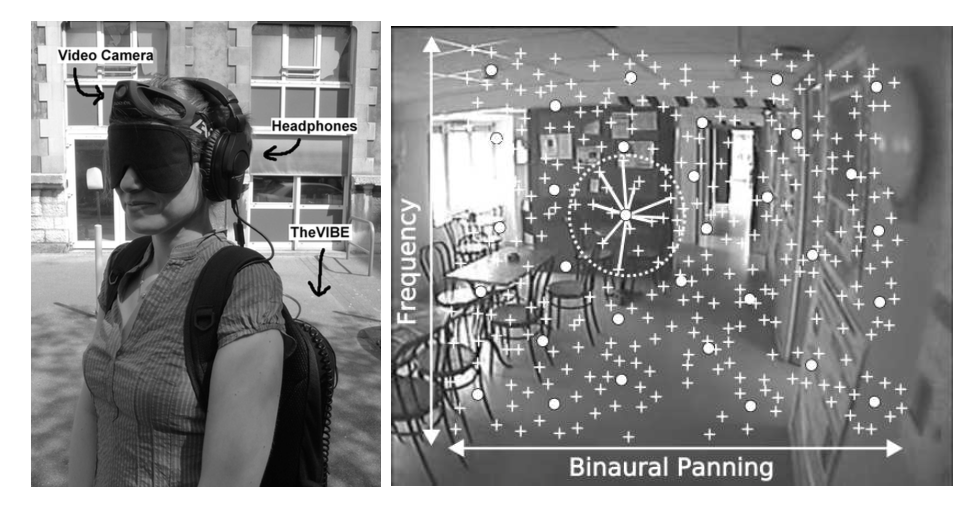
\includegraphics[width=0.5\textwidth]{Background/thevibe.png}
    \caption{Visualisation of point spacing in TheVIBE}
\end{figure}

This paper describes a technique whereby points are assigned to ``receptive fields''. Each field has a static position, and is assigned loudness, determined by the Z-axis position of the points within the field. Unlike the method discussed in section \ref{sec:vas}, TheVIBE does not use a full \ac{HRTF} to convey field position; rather, it uses an inter-aural loudness difference (similar to stereo panning) to describe horizontal position, and tone frequency variation to describe vertical position.

\subsection{EyeMusic}
\subsection{PSVA}

\subsection{Summary of disadvantages of existing solutions}
